%!TEX root = ../../fourthYearReport.tex


\paragraph{Work package 4 progress}

The progress for each task are described hereafter.

\subparagraph*{Improved Models from Real-Time Regression with Latent Contact Type Inference (T4.1)}

%!TEX root = ../../thirdYearReport.tex


Within T4.1 IIT developed a theoretical framework for estimating whole-body
dynamics from distributed multimodal sensors \cite{Nori2015}. Considered sensors
include joint encoders, gyroscopes, accelerometers and force/torque sensors.
Estimated quantities are position, velocity, acceleration and (internal and
external) wrenches on all the rigid bodies composing the robot articulated
chain. The estimation procedure consists of an extended Kalman filter (EKF)
which gives the a-posteriori estimation given all the available measurements.
Computational efficiency is obtained by formulating the Kalman filter
update-step with a sparse Bayesian network. Experiments for validating the
proposed theoretical framework have been conducted on a leg of the iCub humanoid
robot. The iCub is an ideal platform for the proposed experiment given its
distributed force, torque, linear acceleration and angular velocity sensors.
Results have shown the accuracy and the computational efficiency of the proposed
method. The theoretical framework has been implemented in an open source
software (see also Section \ref{sec:T15}).

\subparagraph*{Inferring the Operational Space and Appropriate Controls with Multiple Contacts (T4.2)}

%\subparagraph*{Inferring the Operational Space and Appropriate Controls with Multiple Contacts (T4.2)}

\textbf{Objective}

Accurate sensing of joint angles is a crucial requirement for effective dynamic whole-body control of humanoid robots. While, for standard robot platforms, some kinematic parametric models are typically extracted from the CAD diagrams, joint encoders offsets are assembly dependent. Therefore, the accurate calibration of such parameters is required after any repair task, and can be frequent. For that reason, a fast, accurate, automatic and in-situ method for calibrating joint encoders offsets was identified as a real necessity within the WP4 research scope. A method was proposed using multiple on-board inertial sensors. The method consists in aligning, for each accelerometer, the sensor measurements with the expected link acceleration vector expressed on the sensor frame. The computation of the expected link acceleration depends on the forward kinematics, including the joint offsets. The problem can then be posed as an over-constrained nonlinear least squares minimization process.

\textbf{Innovation}

Prior methods have been proposed in the same context: some use external kinematic constraints \cite{Hollerbach2008} \cite{Liu2009}; others use, as we do, inertial sensors and least-squares optimisation but focus on full kinematic parameters estimation, require specific recursive sequence of complex motion patterns, the accelerometers cross-axis sensitivity is not estimated and the calibration can only be performed joint by joint \cite{Wieser2011} \cite{Mittendorfer2012} \cite{Mittendorfer2014}. In contrast, the method we've proposed is novel in that: it doesn't require any external fixture or kinematic constraint, and thus is well suited for field deployments; the input data is acquired in a single slow motion and minimal sequence (we can assume that the measured acceleration is due only to gravity); the calibration is then done in a single optimization process for the complete set of joint encoders offsets; the accelerometers are fully calibrated in-situ within the same automated process (axis gains and cross-axis sensivity due to manufacturing tolerance); we take advantage of the a priori knowledge of the relative pose of each accelerometer with respect to its support link frame, extracted from the CAD diagrams. The calibration can also be done in a chain-wise fashion, independently for each limb.

\textbf*{Implementation:}
The minimization process is based on a cost function evaluating the gap between the measured and the expected gravity acceleration. The method was implemented on Matlab, using the Matlab Optimization Toolbox solver lsqnonlin along with the trust-region-reflective algorithm. The accelerometers  have been calibrated assuming that the sensor model is affine and using an ellipsoid fitting open source tool. Further more, a full diagnosis feature has been implemented for the cross validation of the computed calibration parameters. The tool is based on the same key performance indicators used for calibrating the sensors, and it plots: the distribution of the error on the measured accelerations magnitude; the time series and distribution of the angle between the measured and the expected accelerations; the fitting of the inertial sensor model to its manifold.

\textbf{Main Results}

The training data acquisition, the calibration procedure and the diagnosis/plotting tool have been integrated into a full Matlab application as a single script with a simplified user interface, suited for production teams or researchers using the iCub platform. The application has been validated on Gazebo simulation by using virtual ground truth joint encoders. For that purpose, we implemented a Gazebo-Yarp plugin emulating the iCub skin accelerometers measurements on the yarp interface. the application estimated the joint offsets from the inertial measurements with an accuracy of 0.005 degrees.
The application was tested on an iCub v2.5 fully equiped with the skin inertial sensors. The legs, torso and head inertial sensors and joint encoders were successfuly calibrated. The computed joint offsets were compared against the offsets measured manually, showing a gap always below 2 degrees. Furthermore, the angle error between the measured and the estimated gravity vector across all the inertial sensors is within 3 degrees, as we can see in figure \ref{fig:T4.2-selfCalibration-Diagnosis.png}, this error has been overall reduced by an average factor of 3. This performance should be improved in a future work by fine tuning the sensors orientation frames.
Furthermore, a formal analysis of the accuracy and observability will be performed in the next steps. The proposed method and initial results have been published as a paper \cite{GuedelhaSelfCalibJointOffsets2016} through the 2016 IEEE-RAS International Conference on Humanoid Robots. The application is being released on the github repository \url{https://github.com/robotology-playground/joint-offset-calib-inertial}.



\begin{figure}[hb!]
  \centering
    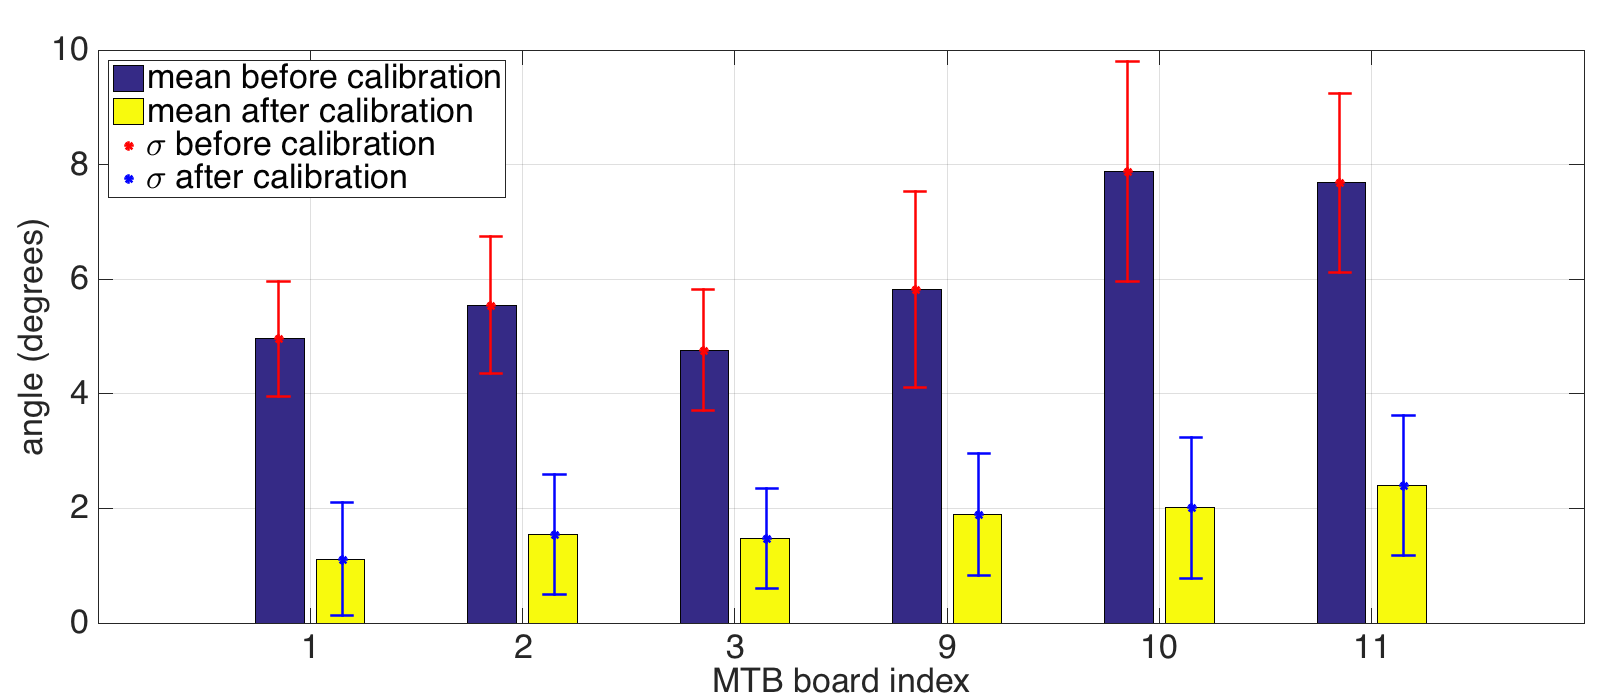
\includegraphics[width=0.8\textwidth]{images/T4.2-selfCalibration-Diagnosis.png}
    \caption{Diagnosis before and after calibration of the left leg joint encoders (angle of accelerometers measurements vs predictions)}
    \label{fig:T4.2-selfCalibration-Diagnosis}
\end{figure}



@inproceedings{GuedelhaSelfCalibJointOffsets2016,
	Author = {Guedelha, Nuno and Kuppuswamy, Naveen and Traversaro, Silvio and Nori, Francesco},
	Booktitle = {Humanoid Robots (Humanoids), 16th IEEE-RAS International Conference on},
	Owner = {nunoguedelha},
	Timestamp = {2016.08.1},
	Title = {Self-calibration of Joint Offsets for Humanoid Robots Using Accelerometer Measurements},
	Year = {2016}}


@incollection{Hollerbach2008,
	Author = {Hollerbach, John and Khalil, Wisama and Gautier, Maxime},
	Booktitle = {Springer Handbook of Robotics},
	Owner = {naveenoid},
	Pages = {321--344},
	Publisher = {Springer},
	Timestamp = {2016.02.18},
	Title = {Model identification},
	Year = {2008}}

@inproceedings{Liu2009,
	Author = {Liu, Yong and Xi, Ning and Zhang, George and Li, Xiongzi and Chen, Heping and Zhang, Chi and Jeffery, Michael J and Fuhlbrigge, Thomas A},
	Booktitle = {Intelligent Robots and Systems, 2009. IROS 2009. IEEE/RSJ International Conference on},
	Organization = {IEEE},
	Owner = {naveenoid},
	Pages = {715--720},
	Timestamp = {2016.02.19},
	Title = {An automated method to calibrate industrial robot joint offset using virtual line-based single-point constraint approach},
	Year = {2009}}


@inproceedings{Wieser2011,
	Author = {Wieser, Erhard and Mittendorfer, Philipp and Cheng, Gordon},
	Booktitle = {Humanoid Robots (Humanoids), 2011 11th IEEE-RAS International Conference on},
	Organization = {IEEE},
	Owner = {naveenoid},
	Timestamp = {2016.02.17},
	Title = {Accelerometer based robotic joint orientation estimation},
	Year = {2011}}


@inproceedings{Mittendorfer2012,
	Author = {Mittendorfer, Philipp and Cheng, Gordon},
	Booktitle = {Robotics and Automation (ICRA), IEEE International Conference on},
	Organization = {IEEE},
	Owner = {naveenoid},
	Pages = {4539--4545},
	Timestamp = {2016.02.17},
	Title = {Open-loop self-calibration of articulated robots with artificial skins},
	Year = {2012}}


@inproceedings{Mittendorfer2014,
	Author = {Mittendorfer, Philipp and Dean, Emmanuel and Cheng, Gordon},
	Booktitle = {Humanoid Robots (Humanoids), 14th IEEE-RAS International Conference on},
	Organization = {IEEE},
	Owner = {naveenoid},
	Timestamp = {2016.02.17},
	Title = {Automatic robot kinematic modeling with a modular artificial skin},
	Year = {2014}}


\end{document}



\subparagraph{Learning the Prioritization of Tasks (T4.4) (TUD: 4PM)}

TUD continued its research on learning task prioritizations from human demonstrations using probabilistic models. This work is currently under review and 
a draft of the paper was added to Deliverable D4.3 in Section 5.  Here is a short summary of the approach. 

Movement prioritization is a common approach
to combine controllers of different tasks for redundant robots.
Each task is assigned a priority, where either strict or 'soft'
priorities can be used. While movement prioritization is an
important concept in the control of whole body movements, it
has been less considered in learning-based approaches, where
prioritization allows us to learn different tasks for different
end-effectors, and subsequently reproduce an arbitrary, unseen
combination of these tasks. This paper combines Bayesian task
prioritization, a 'soft' prioritization technique, with probabilistic
movement primitives to prioritize full motion sequences.
Probabilistic movement primitives can encode distributions of
movements over full motion sequences and provide control
laws to exactly follow these distributions. The probabilistic
formulation allows for a natural application of Bayesian task
prioritization. We demonstrate how the 'soft' priorities can
be obtained from imitation learning and that our prioritized
learning architecture can reproduce unseen task-combinations.
Moreover, we require less data to learn a combination of tasks
than the traditional approach that directly models each task in
joint space. We evaluate our approach on reaching movements
under constraints with a redundant bi-manual planar robot
and the humanoid robot iCub. 

\subparagraph{Learning the Prioritization of Tasks (T4.4) (INRIA: 4.02PM)}

INRIA continued its research on automatically learning soft task priorities (or task weights) using stochastic optimization algorithms. The research is presented in Deliverable D4.3. 

The motivation for the work was to provide an automatic way of determining the temporal profile of the soft task priorities, that are classically manually tuned by experts. When done manually, the critical issue is to define the task transitions, i.e., to define when a task becomes ``less important'' and its weight diminishes, and viceversa.

In a first paper \cite{Modugno_PICRA_2016}, in collaboration with TUD, we investigated how to learn the temporal profile of the soft task priorities (or task weights) in a reinforcement learning scenario. We represented the soft task priorities with parametrized weight functions, and used CMA-ES (Covariance Matrux Adaptation Evolution Strategy, a state-of-the-art blakc-box stochastic optimization algorithm) to optimize their parameters. We showed on a simulated and real robot manipulators that our method was able to obtain better performing solutions that the classic hand-tuned Generalized Hierarchical Controller (developed in WP3).

In a second paper \cite{modugno2016learning} we focused on learning soft task priorities while guaranteeing that the generated behaviors are ``safe'', i.e., that they never violate any of the constraints of the robot and of the system. Indeed, CMA-ES was chosen because of its good exploration properties and ease of use (very few parameters to tune), however it does not take into account constraints violations during the exploration. In \cite{Modugno_PICRA_2016}, the solutions that were not feasible were simply discarded. In \cite{modugno2016learning} we investigated constrained stochastic optimization algorithms, focusing on three variants of CMA-ES: CMA-ES with vanilla constraints, CMA-ES with adaptive constraints and (1+1)-CMA-ES with covariance constrained adaptation. We compared the three algorithms on different benchmarks: classical constrained optimization problems with known solutions and two constrained robotics problems of our design. We found that the third method satisfies our requirements, specifically it always leads to solutions that never violate constraints. We showed the effectiveness of the approach by generating safe whole-body behaviors of iCubNancy01.

\subparagraph{Task compatibility optimization (T4.4) (UPMC: 1.87PM)}

As part of WP4 and WP3, UPMC has worked on improving its approach for task compatibility optimization. Indeed, highly redundant robots, such as humanoids, can execute multiple simultaneous tasks allowing them to perform complex whole-body behaviors. Unfortunately, tasks are generally planned without close consideration for the underlying controller being used, or the other tasks being executed. Because of this, tasks are often incompatible with one another and/or the system constraints, and cannot always be accomplished simultaneously. These incompatibilities can be managed using prioritization and gains, but tuning them is tedious. In this work, an alternative approach is taken and a task compatibility optimization loop which automatically improves task compatibility by modifying their trajectories using reinforcement learning is developed. To do so, the tasks are iteratively optimized by minimizing a compatibility cost, which measures the compatibility between one or more tasks, and the system constraints. Using two common scenarios, It is shown that task compatibility optimization results in whole-body behaviors which better match the original intent of the task combination without the need for manual tuning of task/controller parameters, heuristics, or re-planning. These results extend the contributions \cite{lober-HUMANOIDS2014} and \cite{lober_IROS2015} both in terms of achieved performances and computational efficiency. This work is described in \cite{deliverable33} and was submitted for presentation at a robotics journal~\cite{lober2017RAL-IROS}.

